\documentclass[tikz,border=2pt,11pt]{standalone}
\usetikzlibrary{arrows.meta}
\usetikzlibrary{decorations.pathreplacing}
\usetikzlibrary{patterns}
\usetikzlibrary{calc}
\usepackage{amsmath}
\usepackage{amssymb}
\usepackage{bm}
\usepackage{graphicx}
\usepackage{tikz}
\usepackage{xcolor}
\newcommand{\R}{\mathbb R}
\newcommand{\N}{\mathbb N}
\newcommand{\Q}{\mathbb Q}
\newcommand{\C}{\mathbb C}
\newcommand{\dd}{\,\mathrm d}
\newcommand{\supp}{\operatorname{supp}}
\newcommand{\Tr}{\operatorname{Tr}}
\newcommand{\poly}{\operatorname{poly}}
\newcommand{\dist}{\operatorname{dist}}
\newcommand{\diag}{\operatorname{diag}}
\newcommand{\Spec}{\operatorname{Spec}}
\begin{document}
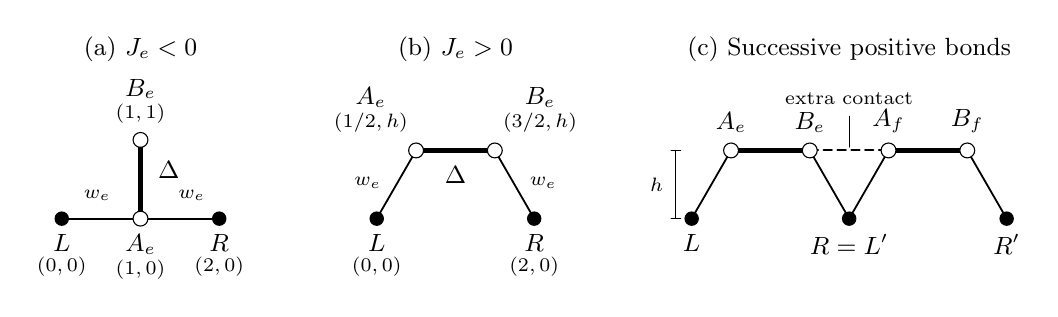
\begin{tikzpicture}[
 x=1cm,y=1cm,line cap=round,
 original/.style={circle,fill=black,draw=black,inner sep=1.7pt},
 ancilla/.style={circle,fill=white,draw=black,inner sep=1.9pt},
 weak/.style={line width=0.65pt},
 strong/.style={line width=1.5pt},
 extra/.style={densely dashed,line width=0.75pt},
 every node/.style={font=\small}]
 \begin{scope}
  \node at (1,2.15) {(a) $J_e<0$};
  \draw[weak] (0,0)--(1,0)--(2,0);
  \draw[strong] (1,0)--(1,1);
  \node[original] at (0,0) {};
  \node[original] at (2,0) {};
  \node[ancilla] at (1,0) {};
  \node[ancilla] at (1,1) {};
  \node[anchor=north] at (0,-0.08)
       {\shortstack{$L$\\[-1pt]\scriptsize$(0,0)$}};
  \node[anchor=north] at (1,-0.08)
       {\shortstack{$A_e$\\[-1pt]\scriptsize$(1,0)$}};
  \node[anchor=north] at (2,-0.08)
       {\shortstack{$R$\\[-1pt]\scriptsize$(2,0)$}};
  \node[anchor=south] at (1,1.08)
       {\shortstack{$B_e$\\[-1pt]\scriptsize$(1,1)$}};
  \node[anchor=west] at (1.10,0.62) {$\Delta$};
  \node[font=\scriptsize,anchor=south] at (0.45,0.10) {$w_e$};
  \node[font=\scriptsize,anchor=south] at (1.65,0.10) {$w_e$};
 \end{scope}
 \begin{scope}[shift={(4,0)}]
  \node at (1,2.15) {(b) $J_e>0$};
  \draw[weak] (0,0)--(0.5,0.8660254);
  \draw[weak] (1.5,0.8660254)--(2,0);
  \draw[strong] (0.5,0.8660254)--(1.5,0.8660254);
  \node[original] at (0,0) {};
  \node[original] at (2,0) {};
  \node[ancilla] at (0.5,0.8660254) {};
  \node[ancilla] at (1.5,0.8660254) {};
  \node[anchor=north] at (0,-0.08)
       {\shortstack{$L$\\[-1pt]\scriptsize$(0,0)$}};
  \node[anchor=north] at (2,-0.08)
       {\shortstack{$R$\\[-1pt]\scriptsize$(2,0)$}};
  \node[anchor=south east] at (0.52,0.97)
       {\shortstack{$A_e$\\[-1pt]\scriptsize$(1/2,h)$}};
  \node[anchor=south west] at (1.48,0.97)
       {\shortstack{$B_e$\\[-1pt]\scriptsize$(3/2,h)$}};
  \node[anchor=north] at (1,0.79) {$\Delta$};
  \node[font=\scriptsize,anchor=east] at (0.18,0.45) {$w_e$};
  \node[font=\scriptsize,anchor=west] at (1.82,0.45) {$w_e$};
 \end{scope}
 \begin{scope}[shift={(8,0)}]
  \node at (2,2.15) {(c) Successive positive bonds};
  \draw[weak] (0,0)--(0.5,0.8660254);
  \draw[weak] (1.5,0.8660254)--(2,0)--(2.5,0.8660254);
  \draw[weak] (3.5,0.8660254)--(4,0);
  \draw[strong] (0.5,0.8660254)--(1.5,0.8660254);
  \draw[strong] (2.5,0.8660254)--(3.5,0.8660254);
  \draw[extra] (1.5,0.8660254)--(2.5,0.8660254);
  \foreach \x in {0,2,4} {\node[original] at (\x,0) {};}
  \foreach \x in {0.5,1.5,2.5,3.5}
       {\node[ancilla] at (\x,0.8660254) {};}
  \node[anchor=north] at (0,-0.08) {$L$};
  \node[anchor=north] at (2,-0.08) {$R=L'$};
  \node[anchor=north] at (4,-0.08) {$R'$};
  \node[anchor=south] at (0.5,0.97) {$A_e$};
  \node[anchor=south] at (1.5,0.97) {$B_e$};
  \node[anchor=south] at (2.5,0.97) {$A_f$};
  \node[anchor=south] at (3.5,0.97) {$B_f$};
  \draw[thin] (-0.2,0)--(-0.2,0.8660254);
  \draw[thin] (-0.26,0)--(-0.14,0);
  \draw[thin] (-0.26,0.8660254)--(-0.14,0.8660254);
  \node[anchor=east,font=\scriptsize] at (-0.24,0.433) {$h$};
  \draw[thin] (2,1.30)--(2,0.91);
  \node[font=\scriptsize,anchor=south] at (2,1.32)
       {extra contact};
 \end{scope}
\end{tikzpicture}
\end{document}
